\documentclass[
	%a4paper, % Use A4 paper size
	letterpaper, % Use US letter paper size
]{jdf}
\newcommand{\pcite}[1]{(\cite{#1})}
\addbibresource{../../references.bib}
\author{William Luna}
\email{wluna6@gatech.edu}
\title{Assignment 3: Research Log}

\begin{document}
%\lsstyle

\maketitle

\section{Background}
% In about half a page, summarize your current state. This would largely cover where you left off last week.
The research from last week brought a great deal of clarity to what I want to focus on. To summarize the core learnings of the last two weeks:
\begin{enumerate}
    \item Vocabulary acquisition is an important part of language learning,
    \item Extensive Reading is a helpful exercise in acquiring new vocabulary,
    \item Using a dictionary during extensive reading has a neutral to positive impact on acquiring new vocabulary,
    \item New vocabulary is most efficiently transferred into long-term memory when prompted for recall at increasing intervals, and
    \item Extensive reading is a potential vehicle for prompting recall of newly acquired vocabulary.
\end{enumerate}

This is a very formal way of pointing out what is perhaps quite obvious: we read books, look up new words when we don't recognize them, and can bet that the same book will use those new words enough to cement them into our long-term memory.    

Almost all of the papers reviewed in the last two weeks either provide evidence for one of the numbered statements above, or address a challenge in implementing them, such as "how to best provide extensive reading material to beginners?", "are monolingual or bilingual dictionaries more effective?", or "what is the most efficient algorithm for spaced repetition?" This also includes an exploration into technical implementation, such as which spaced repetition algorithm is the most effective, whether an LLM or more traditional machine learning algorithm is suited for text generation, etc. 

In the process of shoring up my understanding of the learning science, I came across some important, novel concepts. This week's papers are focused on \textbf{controllable story generation} (particular using LLMs), \textbf{knowledge tracing}, the \textbf{zone of proximal development}, and a couple of recently discovered language learning products, notably Prismatext (\textbf{diglot weave}) and Hyplern (\textbf{interlinear glossing}).

\section{Papers and Other Reference Material}
%As you walk through the Research Guide, you’ll be finding lots of papers to read. Here, you’ll make a list of the papers you come across and give considerable attention to. We would expect the Research Log to include at least 15-20 sources (though more is fine as well), and at least 12 (preferably more) should be academic and peer-reviewed. You may include blog posts, newspaper articles, etc. as well, but you should have at least 12 academic sources, too.

\subsection{\fullcite{ye2023storypark}}

%In around one sentence, how you found it (a Google Scholar search? From a conference’s proceedings? From another paper’s references? %Something else?)
Asked Chat GPT to provide papers that leverage LLMs for language learning applications. Interestingly, it hallucinated, providing the name of a paper that doesn't exist, but this was the top result returned by Google when typing in the fake paper's name.

\subsubsection{Summary}
%In around three sentences, a brief, original summary in your own words
This paper evaluates the capacity of GPT-3 to enable interactive storytelling with children. A simple storytelling AI is constructed with prompt engineering wrapped around the GPT, and it is embedded into an iPad application where a child is asked to provide details about a story that inform the future narrative. An experiment is administered where children interact with two versions of the app, one where story continuity is generated by the GPT and another where it is generated by a human. Child develpment experts rate the resulting stories on indices of creativity, interaction, comprehensibility, and other factors. The GPT is found to perform only slightly worse than the human storytellers.

\subsubsection{Takeaways}
%In around three sentences, the main takeaways going forward
This is one of the first papers I've read that leverage a GPT to incorporate to a reader/listener's feedback into the subsequent parts of the story it is telling. However, it does not consider language learning a core component of the research. My main takeaway is actually the use of solely qualitative feedback in the papers analysis, results, and conclusions section. While I may agree that the qualitative feedback of human experts is superior to an assessment generated by a machine learning model, evaluation metrics for LLM output were well-defined when this paper was published, making the reason for their absence unclear.

\subsection{\fullcite{llmtutor}}
%In around one sentence, how you found it (a Google Scholar search? From a conference’s proceedings? From another paper’s references? %Something else?)
I made a generic Google Scholar search exploring how LLMs have most recently been leveraged in the context of language learning.

\subsubsection{Summary}
%In around three sentences, a brief, original summary in your own words
This paper includes a literature review, a refresher on multiple theories of learning, introduces different prompts to train an LLM at several tasks, uses an evaluation framework to grade the LLMs' performance, runs an experiment, and evaluates the results along quantitative and qualitative benchmarks. All in six pages. 

\subsubsection{Takeaways}
%In around three sentences, the main takeaways going forward
I felt this paper was rather impenetrable, my biggest takeaway being that the importance of a paper's length matching the ambition of its scope. The consequence was a paper with no obvious conclusions. This paper being on arxiv, it's possible that it's still in development. If so, this is a cautionary tale about sacrificing peer review in order to read the most recent papers that discuss bleeding-edge LLMs.

\subsection{\fullcite{vygotsky}}
%In around one sentence, how you found it (a Google Scholar search? From a conference’s proceedings? From another paper’s references? %Something else?)
Vygotsky's theory of the Zone of Proximal Development came up in the literature overview of the paper above and Chapter Six of this book is where the term was coined.

\subsubsection{Summary}
%In around three sentences, a brief, original summary in your own words
The chapter begin with an overview of competing definitions of learning, development, and how the two concepts interact, especially in regards to early childhood education. Vygotsky proceeds to reject all previously discussed theories in favor of the Zone of Proximal Development, which he defines as "\textit{the distance between the actual developmental level as determined by independent problem solving and the level of potential development as determined through problem solving under adult guidance or in collaboration with more capable peers}" (emphasis his). There's additional discussion of how development of children is radically different before and after they are of schooling age.

\subsubsection{Takeaways}
%In around three sentences, the main takeaways going forward
Vygotsky's theory interests me from the perspective that the Zone of Proximal Development appears to be analogous to, or at least complementary to, Krashen's theory of Massive Comprehensible input (i+1). Both rest make the claim that learning is best performed when students are asked to reach \textit{just} beyond their cognitive grasp. However, it's unclear if this conclusion has consensus in the scientific community or is my own unique conclusion biased from limited exposure to the field.

\subsection{\fullcite{vygostky_krashen_not_same}}
%In around one sentence, how you found it (a Google Scholar search? From a conference’s proceedings? From another paper’s references? %Something else?)
I wanted to pull on the thread of the above takeaway and asked Chat GPT to provide papers that explore the similarities and differences between Krashen's and Vygotsky's theories.

\subsubsection{Summary}
%In around three sentences, a brief, original summary in your own words
The paper covers the history of comparisons between Krashen's i+1 and Vygotsk''s ZPD, from a 1983 paper that directly conflates the two ("'near the student's "zone of proximal development" or "i+1"'") up through a (then contemporary) 1996 paper that also equates them ("'the i+1 stage is equivalent to Vygotsky's zone of proximal development'"). The author then deems the two theories "superficially similar" but "profoundly different" mostly on the grounds that Krashen and Vygotsky had profoundly different views on how learning intersects with development, and that Krashen's theories don't transfer well to domains outside of language acquisition.

\subsubsection{Takeaways}
%In around three sentences, the main takeaways going forward
This is a fascinating thread of academic inquiry, but I'm going to stop here since further understanding of the nuance won't do much to inform the direction of my project. The major learning of this argument is that Vygotsky's frameworks shouldn't be assumed to relate to Krashen's by default, meaning that I should not dig into current literature on his work as a new font of complementary ideas.

\subsection{\fullcite{controllable_story_generation}}
%In around one sentence, how you found it (a Google Scholar search? From a conference’s proceedings? From another paper’s references? %Something else?)
I asked Chat GPT the following:

\blockquote{I have an idea to leverage an LLM to continuously generate new parts of a story, where a key goal of the LLM is to 1) produce text that is at the reader's level and 2) uses new vocabulary in the story according to a spaced repetition program. To elaborate, the idea is that the reader clicks on which words they do not understand, which are then added to word bank, where each word in this word bank should be presented at the ideal interval in the text generated by the LLM.

I know LingQ as a product provides well graded reading content and can add unknown words to a flashcard deck. But to my knowledge, it and all other products and research are missing the component of dynamically incorporating those unknown words into an evolving story.}

It provided this research paper as a relevant resource while admitting that it does not have an identical goal.

\subsubsection{Summary}
%In around three sentences, a brief, original summary in your own words
This paper proposes the idea of using an LLM to dynamically generate a story based on user input. The introduction walks through the history of the field from Meehan's TALE-SPIN through LSTM-based that even take advantage of Ilya Sutskever's work on encoder-decoder neural networks, the groundwork for Chat GPT. \textit{Controllability} is discussed as an under-examined aspect of AI-based story generation. A model is trained to capture how a story ends-happy, sad, or ambiguous–and is deployed to provide different endings to several unfinished stories.

\subsubsection{Takeaways}
%In around three sentences, the main takeaways going forward
This is a critically helpful paper in my research. It points out that I have under-explored story generation as a body of research. It will be important to see if more recent papers that cite this one more heavily leverage LLMs and/or successfully provide more granual story controls than the emotion of the ending.

\subsection{\fullcite{recent_story_generation_review}}
%In around one sentence, how you found it (a Google Scholar search? From a conference’s proceedings? From another paper’s references? %Something else?)
I pressed Chat GPT on a paper it had probably hallucinated. It offered this as an alternative.

\subsubsection{Summary}
%In around three sentences, a brief, original summary in your own words
This paper provides strong evidence that the latest language models are not only effective at concluding and summarizing stories, but that humans prefer their output over smaller models purpose-built for the task. The paper highlights some challenging edge cases, such as the model occasionally using expletives, responding in a foreign language, or soft plagiarizing existing literary works.

\subsubsection{Takeaways}
%In around three sentences, the main takeaways going forward
This paper surfaces the pitfalls of building any system that generates stochastic output, in that no matter how well it performs in general, there's no guarantee that it won't generate problematic output in a specific instance.

\subsection{\fullcite{ai_human_taking_turns_creating_story}}
%In around one sentence, how you found it (a Google Scholar search? From a conference’s proceedings? From another paper’s references? %Something else?)
Chat GPT offered this paper as an additional alternative to the one it hallucinated.

\subsubsection{Summary}
%In around three sentences, a brief, original summary in your own words
Researchers fine-tune a publicly-available LLM on top of writing prompts and corresponding fictional works generating from those prompts. This LLM is then deployed as a game, where it starts the story, waits for a human to continue, the story, adds to the story itself, and repeats this process until the human concludes the story. Mechanical Turk workers were asked to rate the continuity of stories generated by both the fine-tuned version of the model and the default LLM, soliciting pairwise user preferences. There is strong evidence that the fine-tuned model generated output most preferred by humans.

\subsubsection{Takeaways}
%In around three sentences, the main takeaways going forward
This paper's use of story starters echoes my similar idea to start all stories with one of a handful of introductions. It also highlights the challenge in establishing useful evaluation frameworks. In my opinion, the evaluation framework mismatches the goal of the study, since proving that the fine-tuned model outperforms the others does not explicitly validate a user's apetite or overall enthusiasm for the exercise of creating a story together with an AI.

\subsection{\fullcite{taiwan_adaptive_testing}}
%In around one sentence, how you found it (a Google Scholar search? From a conference’s proceedings? From another paper’s references? %Something else?)
Searched for papers on collaborative storytelling on Google Scholar.

\subsubsection{Summary}
%In around three sentences, a brief, original summary in your own words
Paper assesses the feasibility of integrating an LLM into the Taiwan Adaptive Learning Platform, an educational tool established by the country's ministry of education. TALP is described as a tool that asks students questions and based on a hierarchy of skills and knowledge, both drills-down and emphasizes the elements of a quiz the student's answer incorrectly. This is anchored in Vygotsky's socio-cultural theory and Zone of Proximal Development. 

\begin{figure}
    \centering
    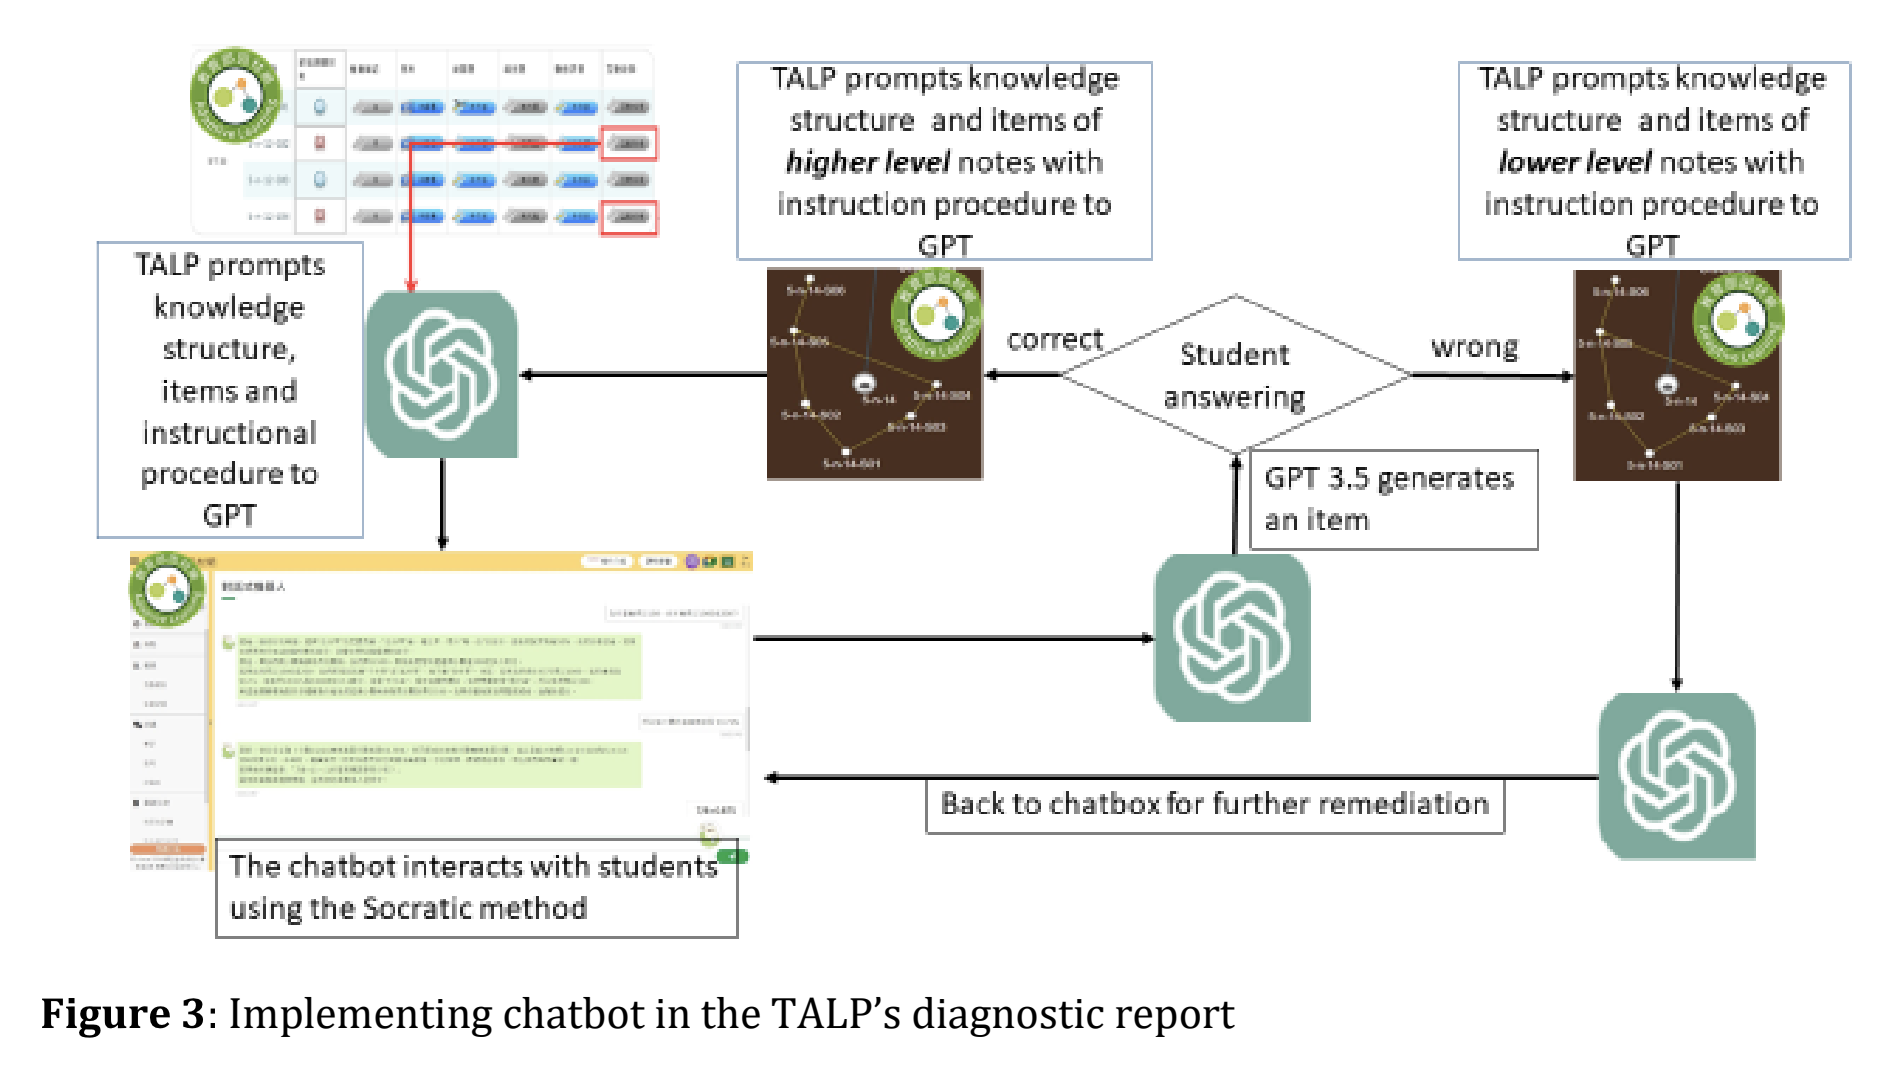
\includegraphics[width=0.5\linewidth]{Assignments//Assignment 3/TALP_GPT.png}
    \caption{: Implementing chatbot in the TALP’s diagnostic report}
    \label{fig:enter-label}
\end{figure}

\subsubsection{Takeaways}
%In around three sentences, the main takeaways going forward
This is an interesting case study on how a top-down, rules-based system (TALP) and a black-box LLM (Chat GPT) can be integrated effectively. This is encouraging, given that I am considering a similar integration (top-down vocabulary SRS system with LLM-driven story generation).

\subsection{\fullcite{important_adaptive_learning_exercise_generation}}
%In around one sentence, how you found it (a Google Scholar search? From a conference’s proceedings? From another paper’s references? %Something else?)
Typed "Adaptive learning" into Google Scholar, since it was used in the terminology of the earlier paper.

\subsubsection{Summary}
%In around three sentences, a brief, original summary in your own words
Introduces adaptive learning as the potentially most fitting label for the topic of this project. Introduces such learning models as having three components, a domain model, a learner model, and an adaptation model, that correspond to the content being studies, a mental model of the student's knowledge, and how the two are combined. Explains the difference between adaptive learning and controlled text generation. Creates a model where the student's performance on past exercises and vocabulary enbles the creation of exercises at an appropriate estimated level of difficulty for that particular student.

\subsubsection{Takeaways}
%In around three sentences, the main takeaways going forward
This paper comes closer to capturing the goals of my project than other. Although to thoughtfully replicate this study, or even leverage all of the core tenets in its knowledge training model, would require far too much work to be achievable this term. The ablation study is a fascinating strategy tease apart which aspect of a model had the greatest impact. This paper should be used as a launching pad into the fields of controlled text generation and adaptive learning. 

\subsection{\fullcite{deep_knowledge_tracing}}
%In around one sentence, how you found it (a Google Scholar search? From a conference’s proceedings? From another paper’s references? %Something else?)
Cited in the above paper.

\subsubsection{Summary}
%In around three sentences, a brief, original summary in your own words
Provides a primer for using a recurrent neural network to model and predict student performance. Historical use of Bayesian modeling for knowledge tracing is discussed, including Hidden Markov models. The paper considers two innovative approached to knowledge tracing, a vanilla RNN and a LSTM, with the RNN method beating the current SOTA approach based on knowledge tracing benchmarks that were also novel to me.

\subsubsection{Takeaways}
%In around three sentences, the main takeaways going forward
An example where a large language model has more obstacles in replacing a neural network, not sure how the student knowledge state would remain observable in an LLM. Creates something of an earthquake of realization for my project–should I be using knowledge tracing to store a representation of student knowledge instead of spaced repetition flashcards? If still necessary to utilize a traditional LLM for content generation, how to blend into a vanilla LLM? I think these technical challenges take the possibility firmly beyond the scope of a project I can hope to finish in this class, however.

\subsection{\fullcite{question_generation_adaptive_education}}
%In around one sentence, how you found it (a Google Scholar search? From a conference’s proceedings? From another paper’s references? %Something else?)
Searched for papers on collaborative storytelling on Google Scholar.

\subsubsection{Summary}
%In around three sentences, a brief, original summary in your own words 
Paper outlines a method of fine-tuning a KT-LM (knowledge tracing language model) to generate questions and predicting the likelihood that the student will answer the question correctly as a proxy for difficulty. This model is trained and tested on a dataset of student prompts and answers from Duolingo and found accuracy to be high enough to conclude this as a viable means of generating translation tasks for second language students. 

\subsubsection{Takeaways}
%In around three sentences, the main takeaways going forward
This paper let me sit with the implementation details of a knowledge tracing model and convinced me that it would not be feasible for this course project. However, in theory this may be the best means of generating a story based on an understanding of the student's vocabulary, optimized to estimate 98 percent known words. There's a chicken and egg problem. With enough training data from a simpler system, it would become possible to train a KT model (Duolingo is a perfect analogy, since it's language tasks remain mostly the product of top-down design).

\subsection{\fullcite{llm_augmented_exercise_retrieval}}

%In around one sentence, how you found it (a Google Scholar search? From a conference’s proceedings? From another paper’s references? %Something else?)
Found by searching for papers that cite \cite{important_adaptive_learning_exercise_generation} via Google Scholar.

\subsubsection{Summary}
%In around three sentences, a brief, original summary in your own words
Focuses on \textit{learner initiated personalization}, under the pretense that giving learners the ability to shape their learning experience drives motivation and self-actualization. The paper proposes a \textit{multilingual Hypothetical Exercise Retriever} (mHyER) that is able to combine an evolving representation of student knowledge with that student's requested activities to suggest activities of that type at the appropriate level. This model has AUC (area under curve) gains over mBert, and mContreiver, which the study considers proof of a new SOTA model.

\subsubsection{Takeaways}
%In around three sentences, the main takeaways going forward
Fascinating to consider the challenge in balancing a tradeoff between optimizing for student learning and agency in these knowledge tracing models. 

\subsection{\fullcite{flashcard_scheduler_evolution}}
%In around one sentence, how you found it (a Google Scholar search? From a conference’s proceedings? From another paper’s references? %Something else?)
Found by searching for papers that cite \cite{important_adaptive_learning_exercise_generation} via Google Scholar.

\subsubsection{Summary}
%In around three sentences, a brief, original summary in your own words
KARL (\textbf{K}nowledge-\textbf{A}ware \textbf{R}etrieval and Representations aid Retention and \textbf{L}earning in Students) is introduced as a system that leverages Deep Knowledge Tracing (see Peich above) to imbue the information from an SRS scheduler with semantic and recall relationships with other words, creating a more comprehensive model of student knowledge. "if a student knows that John Adams is the second American president, the student model should be able to infer that the student can also answer 'Who was the first American president?', even if this question has not been studied." A balance between comprehensiveness in embedding and speed of updating an online neural network is discussed. KARL's performance is on-par with FSRS, an algorithm explored in earlier research logs.

\subsubsection{Takeaways}
%In around three sentences, the main takeaways going forward
This is a preprint submitted to arxiv in February 2024, less than three months ago. The fact that KARL does not handily outperform FSRS, in addition to the extra latency, cost, and complexity in implementing a neural network, provides evidence that FSRS should thankfully be a sufficient memory model implementation for my project. I also found the specificity of the use case for this method surprising–it relies on the assumption that the flashcards have long, semantically-rich explanations rather than the single word translations commonly-found in language learning reviews. This limited application implies that there is an ocean of work on this topic of which I still have no awareness.

\subsection{\fullcite{generative_information_retrieval}}
%In around one sentence, how you found it (a Google Scholar search? From a conference’s proceedings? From another paper’s references? %Something else?)
Found this paper by looking at papers that cited the last three papers discussed above.

\subsubsection{Summary}
%In around three sentences, a brief, original summary in your own words
Provides a literature overview of generative information retrieval, aka information retrieval that leverages LLMS. Document Identifier Design, Incremental Learning, decoding, optimization, scaling, RAG, and benchmarking are all discussed as ongoing challenges in the forty page report. The emerging nature of all these sub-topics is emphasized (preprint less than a month old).

\subsubsection{Takeaways}
%In around three sentences, the main takeaways going forward
This paper is further evidence that using an LLM to store a representation of student knowledge would add too much complexity to a project I have a hope of completing in this class. Although it gives me hope that there will soon be off-the-shelf APIs that abstract many of the challenges presented here.

\subsection{\fullcite{knowledge_tracing_survey}}
%In around one sentence, how you found it (a Google Scholar search? From a conference’s proceedings? From another paper’s references? %Something else?)
This paper was discussed in another student's work which I reviewed during peer feedback.

\subsubsection{Summary}
%In around three sentences, a brief, original summary in your own words
Another literature review of knowledge tracing emphasizing the roots in the 1980s up until the groundbreaking application of deep learning to the problem (see Piech, above). Includes a section dedicated to the datasets most commonly used to benchmark the performance of a knowledge KT model, as well as future research opportunities, notable multi-modal representations, self-supervised learning, and interactive knowledge. Interactive Knowledge Tracing is the prompting of specific questions during "cold start scenarios" to enable the KT model to build a comprehensive understanding of the student's knowledge as quickly as possible.

\begin{figure}
    \centering
    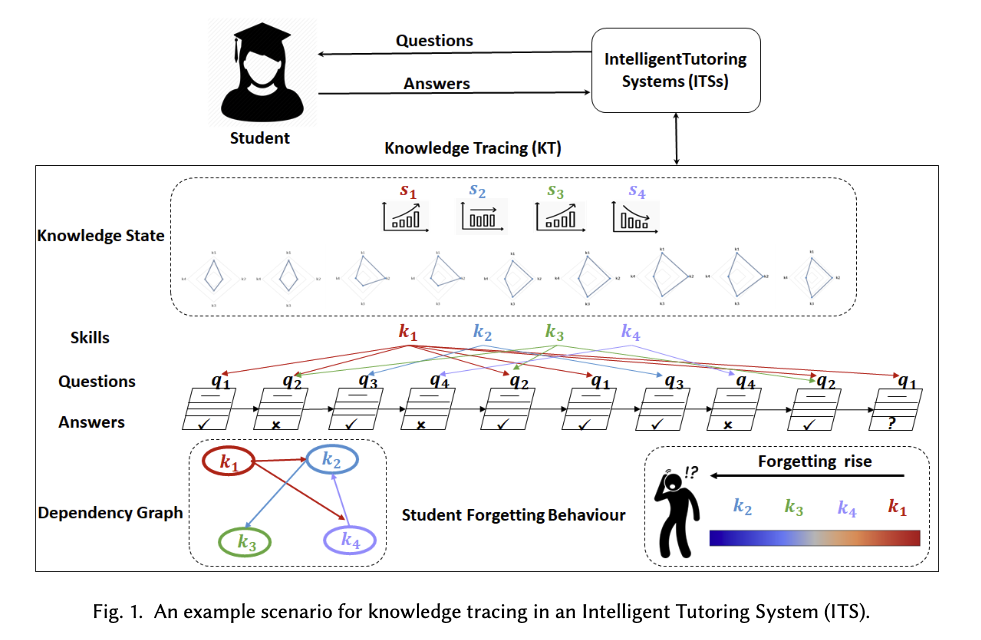
\includegraphics[width=0.5\linewidth]{Assignments//Assignment 3/knowledge_tracing_survey.png}
    \caption{An example scenario for knowledge tracing in an Intelligent Tutoring System (ITS)}
    \label{fig:enter-label}
\end{figure}

\subsubsection{Takeaways}
%In around three sentences, the main takeaways going forward
This was the first time I noticed a palpable difference in paper quality between the pre-prints vs. peer-reviewed publications on arxiv. It forces striking a balance between recency and polish. I wish I read this paper first in the lineage on knowledge tracing. Perhaps a learning to tackle peer reviews \textit{before} the research for the week, since I would have caught this paper much earlier. The clear explanation of how various supervised machine learning models have been applied was helpful (logistic regression, bayesian, etc).

\subsection{\fullcite{deep_learning_knowledge_tracing}}
%In around one sentence, how you found it (a Google Scholar search? From a conference’s proceedings? From another paper’s references? %Something else?)
This paper was discussed in another student's work which I reviewed during peer feedback.

\subsubsection{Summary}
%In around three sentences, a brief, original summary in your own words
Paper mentions differences in adoption rates of intelligent tutoring systems (ITS) across the US and China and provides some reasons for those differences. It also frames the conflict between the adaptive behavior of an ITS versus actionable insights and reporting on student progress, since the first needs accurate predictions and the second emphasises "interpretability and stability." They develop a deep learning model that outperforms baselines on large datasets, but note that simple logistic regression is better on small datasets, and that Markov Models struggle compared to both.

\subsubsection{Takeaways}
%In around three sentences, the main takeaways going forward
Feels like a good place to end investigation into Knowledge Tracing and Intelligent Tutoring Systems. Drew out a curiosity to explore commercial offerings (such as ALEKS by McGraw in the US and Squirrel AI in China). These technologies are rapidly improving and have a high technical ceiling but will be too difficult to implement over the course of this class.

\subsection{\fullcite{dkt_knowledge_tracing}}
%In around one sentence, how you found it (a Google Scholar search? From a conference’s proceedings? From another paper’s references? %Something else?)
This paper was discussed in another student's work which I reviewed during peer feedback.

\subsubsection{Summary}
%In around three sentences, a brief, original summary in your own words
Frames the limitation of traditional knowledge tracing (KT) models as only using the sequence of problems attempted by a student and whether the student was correct or not, losing information about how the problem was attempted. KT is applied to complex learning tasks like logic proofs and scientific inquiry, where this context should matter. Paper reviews the history of KTs applied to CS education, creates a model that includes code2vec embeddings of attempted problems (correct or incorrect) and finds this KT model outperforms a base line without the embeddings.

\subsubsection{Takeaways}
%In around three sentences, the main takeaways going forward
Commonalities are emerging across these KT studies, including use of ablation studies to validate efficacy, the use of recurrent neural networks, and benchmarking via AUC (area under the curve). My main takeaway from this paper is how knowledge tracing models need to be custom designed for a specific domain to be as effective as possible. This model would not have been as successful outside the realm of coding assignments, and also under-performed other models until a sufficient number of attempts had been submitted by the student, which have implications that are hard to objectively evaluate outside the context of the use-case.

\subsection{\fullcite{hyplern_interlinear_reading}}
%In around one sentence, how you found it (a Google Scholar search? From a conference’s proceedings? From another paper’s references? %Something else?)
First result when searching "combining flashcards with extensive reading" on Google.

\subsubsection{Summary}
%In around three sentences, a brief, original summary in your own words
This article does a wonderful job laying out the trade-offs of acquiring vocabulary through extensive reading (in context, slow) vs studying flashcards (out of context, fast). It poses interlinear reading as a best of both worlds solution, where it's possible to read in the target language but with a translation in one's native language in smaller font below each word.

\subsubsection{Takeaways}
%In around three sentences, the main takeaways going forward
I take this blog post as further validation that combining spaced repetition with extensive reading is an acknowledged problem in the language learning community. It's also reassuring to see that there is no elegant proposal to blend both techniques together that approximates my project proposal.

\subsection{\fullcite{diglot_weave}}
%In around one sentence, how you found it (a Google Scholar search? From a conference’s proceedings? From another paper’s references? %Something else?)
A friend recommended Prismatext as a product for language learning and it turned out to be adjacent to the project's objective as well as the other research topics explored so far. It relies on a technique called diglot weave, and this is one of, if not the most, notable research on the method.

\subsubsection{Summary}
%In around three sentences, a brief, original summary in your own words
Experiment presents Iranian students of English with two versions of the same text. One group studied vocabulary through reading texts that used the diglot weave technique–Iranian text that gradually introduces more and more English vocabulary-and and the other used traditional flashcards. The first (experimental group) was found to exhibit higher vocabulary gains at the end of the study period.

\subsubsection{Takeaways}
%In around three sentences, the main takeaways going forward
I believe there are too many flaws in the methodology of this study to draw any meaningful conclusions from its results. The control and experimental groups were hardly exposed to apples-to-apples pedagogy. However, the approach is quite novel, and does present the possibility that diglot weave is a valid means of acquiring vocabulary, especially if student motivation or level for reading entirely in the target language is too low.

\subsection{\fullcite{free_voluntary_reading}}
%In around one sentence, how you found it (a Google Scholar search? From a conference’s proceedings? From another paper’s references? %Something else?)
My mentor recommended I read more Krashen papers and this was cited in \pcite{llm_augmented_exercise_retrieval}.

\subsubsection{Summary}
%In around three sentences, a brief, original summary in your own words
Book published in 2011 with dozens of important observations and summaries of studies on the benefits of free reading. Explores how impact differs across languages, benefits of free vs focused reading, correlation of time spent reading and overall literacy, and reading via the internet, among many other topics. High-level observation that two most important aspects of successful reading is enthusiasm for and access to reading material. Reading correlates to overall vocabulary and literacy level.

\subsubsection{Takeaways}
%In around three sentences, the main takeaways going forward
I will have to read this book in its entirety at some point, fantastic reference and literature review. Its conclusions validate the premise of the project, coming full circle to the first Krashen papers on massive comprehensible input referenced in the first research log.

\section{Synthesis}
%In about a page, summarize the overall body of work you’ve put together. What are the high-level trends, large takeaways, or open questions you’ve found? If you’ve narrowed in on a particular domain, summarize that domain; if you’re still exploring, discuss the overall direction these efforts are leading you toward. Most importantly, anchor this synthesis in the papers you provided above, citing them where appropriate.

The research log begins with historical background on education pedagogy, notably Vygosky's \textbf{Zone of Proximal Development} \pcite{vygotsky}. While I have read papers each week that seem to conflate the two, Krashen's theory of Massive Comprehensible Input (i+1) only maps onto ZPD int jagged, orthogonal ways \pcite{vygostky_krashen_not_same}. Krashen presents several arguments in favor of \textbf{Free Voluntary Reading} as a critical means of vocabulary acquisition \pcite{free_voluntary_reading}.

Then, there's a string of papers that explore the concept of \textbf{Controllable Story Generation}, a field that has existed since the 80s and is concerned with the procedural generation of narratives that conform to expectations inputted by a user. Examples include giving a story a happy or sad ending or variable levels of conclusion in the plot \pcite{controllable_story_generation}. However, there are unique risks in using any stochastic model to generate content for children, since there is risk of expletives, plagiarism, or incomprehensible input \pcite{recent_story_generation_review, ai_human_taking_turns_creating_story}. I concluded that LLMs have been used to generate text to enable storytelling for some time, if few products have been commercialized and/or received widespread adoption in the American K-12 system \pcite{ye2023storypark}.

The research then turned to \textbf{Intelligent Tutoring Systems} (ITS). The Taiwanese Ministry of Education has developed a system that effectively blends the LLM into a top-down learning management system, which makes the bridge between spaced repetition vocabulary presentation and GPT-4 feel like an easier bridge to cross for my own project \pcite{taiwan_adaptive_testing}. A more fitting name for such a system might be \textbf{Adaptive Learning}, which is defined and surveyed in \pcite{important_adaptive_learning_exercise_generation}.

An important subdomain of Adaptive Learning, several papers explore the development of \textbf{Knowledge Tracing} (KT) from supervised machine learning models to recurrent neural networks since a seminal paper in 2015 \pcite{deep_knowledge_tracing}. One paper explores using KT to generate questions tailored to an individual student's knowledge representation, another emphasizes student agency in driving the tutoring content \pcite{question_generation_adaptive_education, llm_augmented_exercise_retrieval}. KT is also proven an effective scheduler of reviews, although performance was not significantly above FSRS scheduling \pcite{flashcard_scheduler_evolution}. Knowledge Tracing can not only select the ideal question or content to put in front of a learner at a given time, but can dynamically generate questions as well \pcite{generative_information_retrieval}. Despite recent progress, many challenges remain, including multi-modal content generation and performing well under "cold start" scenarios where the model has limited learner knowledge \pcite{knowledge_tracing_survey}. There are also trade-offs between the interpretability of a KT model–for teacher's to monitor student progress–and model accuracy that optimizes that student's learning \pcite{deep_knowledge_tracing}. There are additional implementation decisions that are highly context-dependent, such as the subject of instruction (ie computer science vs languages) and the amount of metadata in the learning materials \pcite{dkt_knowledge_tracing}.

The research concludes by examining \textbf{diglot weaves} and \textbf{interlinear reading} as innovations in vocabulary acquisition through reading, but the experiments covering these techniques are too sparse to draw any definitive conclusions from them \pcite{diglot_weave, hyplern_interlinear_reading}.

\section{Reflection}
%In about half a page, reflect on the process of finding sources, reading papers, synthesizing their contents, and building your understanding. What was difficult, and what was easy? What are you finding yourself interested in going forward?
I find it amazing that I was able to continue to find papers and bodies of research that have drastic implications for the project, especially around Adaptive and Personalized Exercise Generation for Online Language Learning. I was not aware of Knowledge Tracing as a research pursuit when starting this class and it has so much depth and relevance that I'm debating a pivot into researching it instead of tackling a project.

In other words, this week has me in agreement with Dr. Joyner that researching a topic is akin to Hercules fighting the hydra: reading one paper usually leads to an awareness of two more relevant papers, creating a seemingly infinite expanse of academia to explore.

\section{Planning}
%In about half a page, provide a plan for what you expect to do next week. What threads or ideas will you pursue? What questions will you seek answers to in the literature?
Given that next week's assignment is to respond to a qualifier question that I don't yet have in hand, it's hard to thoroughly plan for next week. I can only hypothesize that my mentor will produce a qualifier question that challenges some of the assumptions in learning science upon which my project idea rests. This might be exposing a lack of grounding in the learning science of extended reading, for example, or pushing on how knowledge tracing has been integrated into specifically language learning.

My brief foray into diglot weave and interlinear reading at the end of the research log also showed me just how many niche language learning techniques have been embodied through commercial products. The long-tail of language learning applications doesn't surprise me, but the fact that those products take an entirely different approach from the household names of Duolingo and Rosetta Stone certainly does. It would be a helpful exercise to survey these offerings a little deeper. 

%https://www.microsoft.com/en-us/research/wp-content/uploads/2004/06/DynamicLLearning.pdf
%https://www.sciencedirect.com/science/article/pii/S0167639309000430

\printbibliography{}

\end{document}

